% for section-numbered lemmas etc., use "numberwithinsect"
\documentclass[a4paper,english,numberwithinsect]{eurocg18}

% the recommended bibstyle
\bibliographystyle{plainurl}

%------------------------------------------------------------------- 
%if unwanted, comment out or use option "draft"
\usepackage{todonotes}
\usepackage{microtype}
\usepackage[noend, linesnumbered]{algorithm2e}
\usepackage{amsmath}
\usepackage{color}
\usepackage{cite}
\usepackage{pifont}
\usepackage{enumerate}
\usepackage[basic]{complexity}
\usepackage{subcaption}
\usepackage{wrapfig}

% Line numbers are helpful for refereeing
\usepackage[mathlines]{lineno}
\newcommand*\patchAmsMathEnvironmentForLineno[1]{%
\expandafter\let\csname old#1\expandafter\endcsname\csname #1\endcsname
\expandafter\let\csname oldend#1\expandafter\endcsname\csname end#1\endcsname
\renewenvironment{#1}%
     {\linenomath\csname old#1\endcsname}%
     {\csname oldend#1\endcsname\endlinenomath}}%
\newcommand*\patchBothAmsMathEnvironmentsForLineno[1]{%
  \patchAmsMathEnvironmentForLineno{#1}%
  \patchAmsMathEnvironmentForLineno{#1*}}%
\AtBeginDocument{%
\patchBothAmsMathEnvironmentsForLineno{equation}%
\patchBothAmsMathEnvironmentsForLineno{align}%
\patchBothAmsMathEnvironmentsForLineno{flalign}%
\patchBothAmsMathEnvironmentsForLineno{alignat}%
\patchBothAmsMathEnvironmentsForLineno{gather}%
\patchBothAmsMathEnvironmentsForLineno{multline}%
}
\linenumbers

%helpful if your graphic files are in another directory
%\graphicspath{{./graphics/}}

% Author macros::begin %%%%%%%%%%%%%%%%%%%%%%%%%%%%%%%%%%%%%%%%%%%%%%%%
%\newcommand\polylog{{\rm polylog}}

% Author metadata::begin %%%%%%%%%%%%%%%%%%%%%%%%%%%%%%%%%%%%%%%%%%%%%%%%
\title{Maximizing Ink in Symmetric Partial Edge Drawings of $k$-plane Graphs}
%{Maximal Symmetric Partial Edge Drawings With Degree $ > 2$}
%optional, in case that the title is too long; 
%the running title should fit into the top page column
\titlerunning{MaxSPEDs with degree $ > 2$}

%% Please provide for each author the \author and \affil macro, 
%even when authors have the same affiliation, i.e. for each 
%author there needs to be the  \author and \affil macros
\author[1]{Michael H\"oller}
\author[1]{Fabian Klute}
\author[1]{Soeren Nickel}
\author[1]{Martin~N\"ollenburg}
\author[1]{Birgit Schreiber}

\affil[1]{Algorithms and Complexity Group, TU Wien, Vienna, Austria}
%\affil[2]{Algorithms and Complexity Group, TU Wien, Vienna, Austria} %\texttt{fklute@ac.tuwien.ac.at}}
%\affil[3]{Algorithms and Complexity Group, TU Wien, Vienna, Austria \texttt{}}
%\affil[4]{Algorithms and Complexity Group, TU Wien, Vienna, Austria} %\texttt{noellenburg@ac.tuwien.ac.at}}
%\affil[5]{Algorithms and Complexity Group, TU Wien, Vienna, Austria \texttt{}}
%mandatory. First: Use abbreviated first/middle names. 
%Second (only in severe cases): Use first author plus 'et. al.'
\authorrunning{F. Klute and M. N\"ollenburg} 

% Author macros::end %%%%%%%%%%%%%%%%%%%%%%%%%%%%%%%%%%%%%%%%%%%%%%%%%

\newcommand{\martin}[1]{\todo[inline,color=blue!40]{MN: #1}}
\newcommand{\fabian}[1]{\todo[inline,color=pink!40]{FK: #1}}
\newcommand{\birgit}[1]{\todo[inline,color=red!40]{BS: #1}}
\newcommand{\michael}[1]{\todo[inline,color=green!40]{MH: #1}}
\newcommand{\soeren}[1]{\todo[inline,color=orange!40]{SN: #1}}

\newcommand{\ped}{\ensuremath{\textsc{PED}}\xspace}
\newcommand{\maxsped}{\ensuremath{\textsc{MaxSPED}}\xspace}

\begin{document}

\maketitle

\begin{abstract}
	Partial edge drawing (PED) is a drawing style for non-planar graphs, in which edges are drawn only partially as pairs of opposing stubs on the respective end-vertices. 
	In a PED, by erasing the central parts of edges, all edge crossings and the resulting visual clutter are hidden in the undrawn parts of the edges.
	We study symmetric partial edge drawings (SPEDs), in which the two stubs of each edge are required to have the same length. 
	It is known that maximizing the ink (or the total stub length) when transforming a straight-line drawing with crossings into a SPED is generally \NP-hard.
	We show that the problem remains \NP-hard even for 3-plane input drawings.
	For $k$-plane input drawings whose edge intersection graph forms a collection of trees or cacti we present polynomial time algorithms for ink maximization.
\end{abstract}

\section{Introduction}

Visualizing non-planar graphs as node-link diagrams is challenging due to the visual clutter caused by edge crossings. The layout readability deteriorates as the edge density and thus the number of crossings increases.
Therefore alternative layout styles are necessary for non-planar graphs.
A radical approach first used in applied network visualization work by Becker et al.~\cite{bew-vnd-95} is to start with a traditional straight-line graph drawing and simply drop a large central part of each edge and with it many of the edge crossings.
This idea relies on the closure and continuation principles in Gestalt theory, which imply that humans can still see a full line segment based only on the remaining edge stubs by filling in the missing information in our brains.
User studies have confirmed that such drawings remain readable while reducing clutter significantly~\cite{bvkw-epdldge-12,bkl-us-15}.

\begin{wrapfigure}[11]{r}{0.45\textwidth}
	\centering
	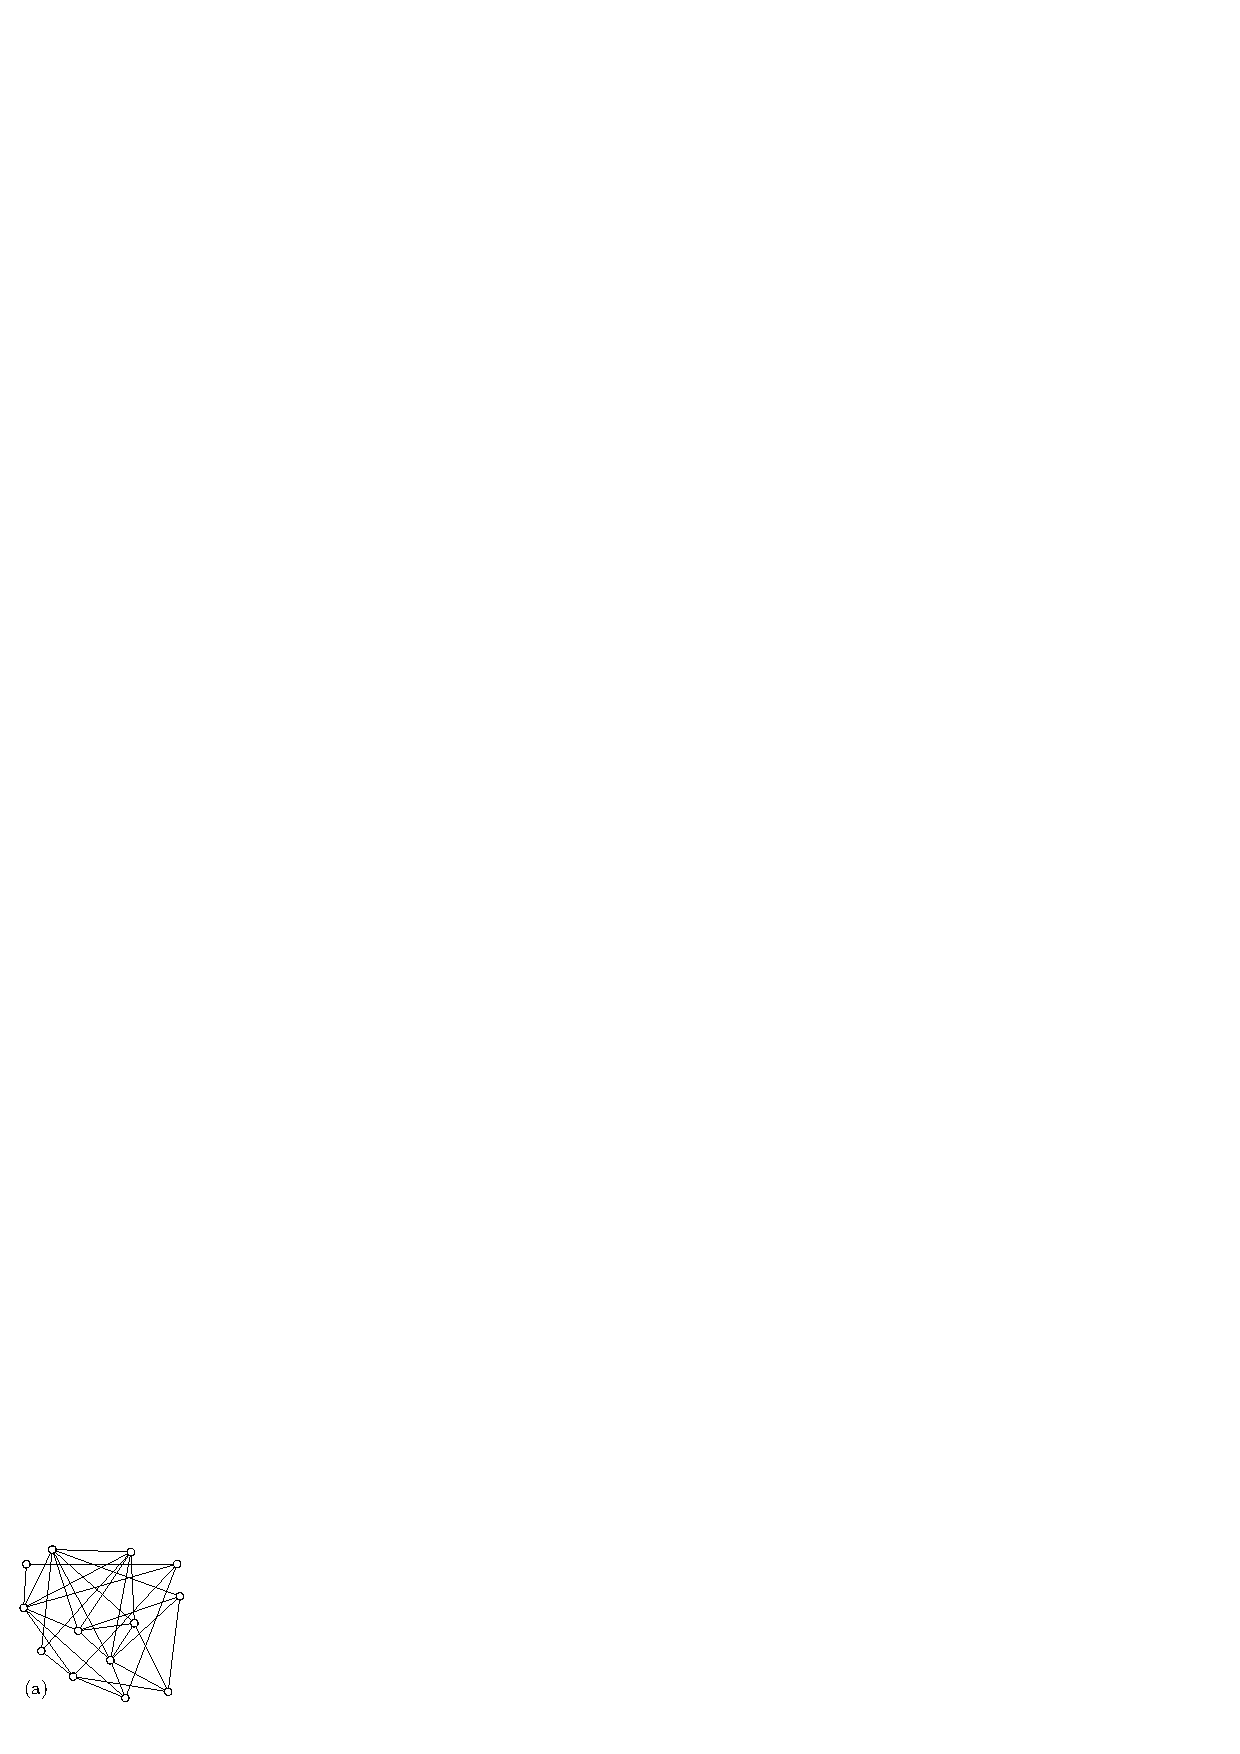
\includegraphics{export_full}
	\hfill
	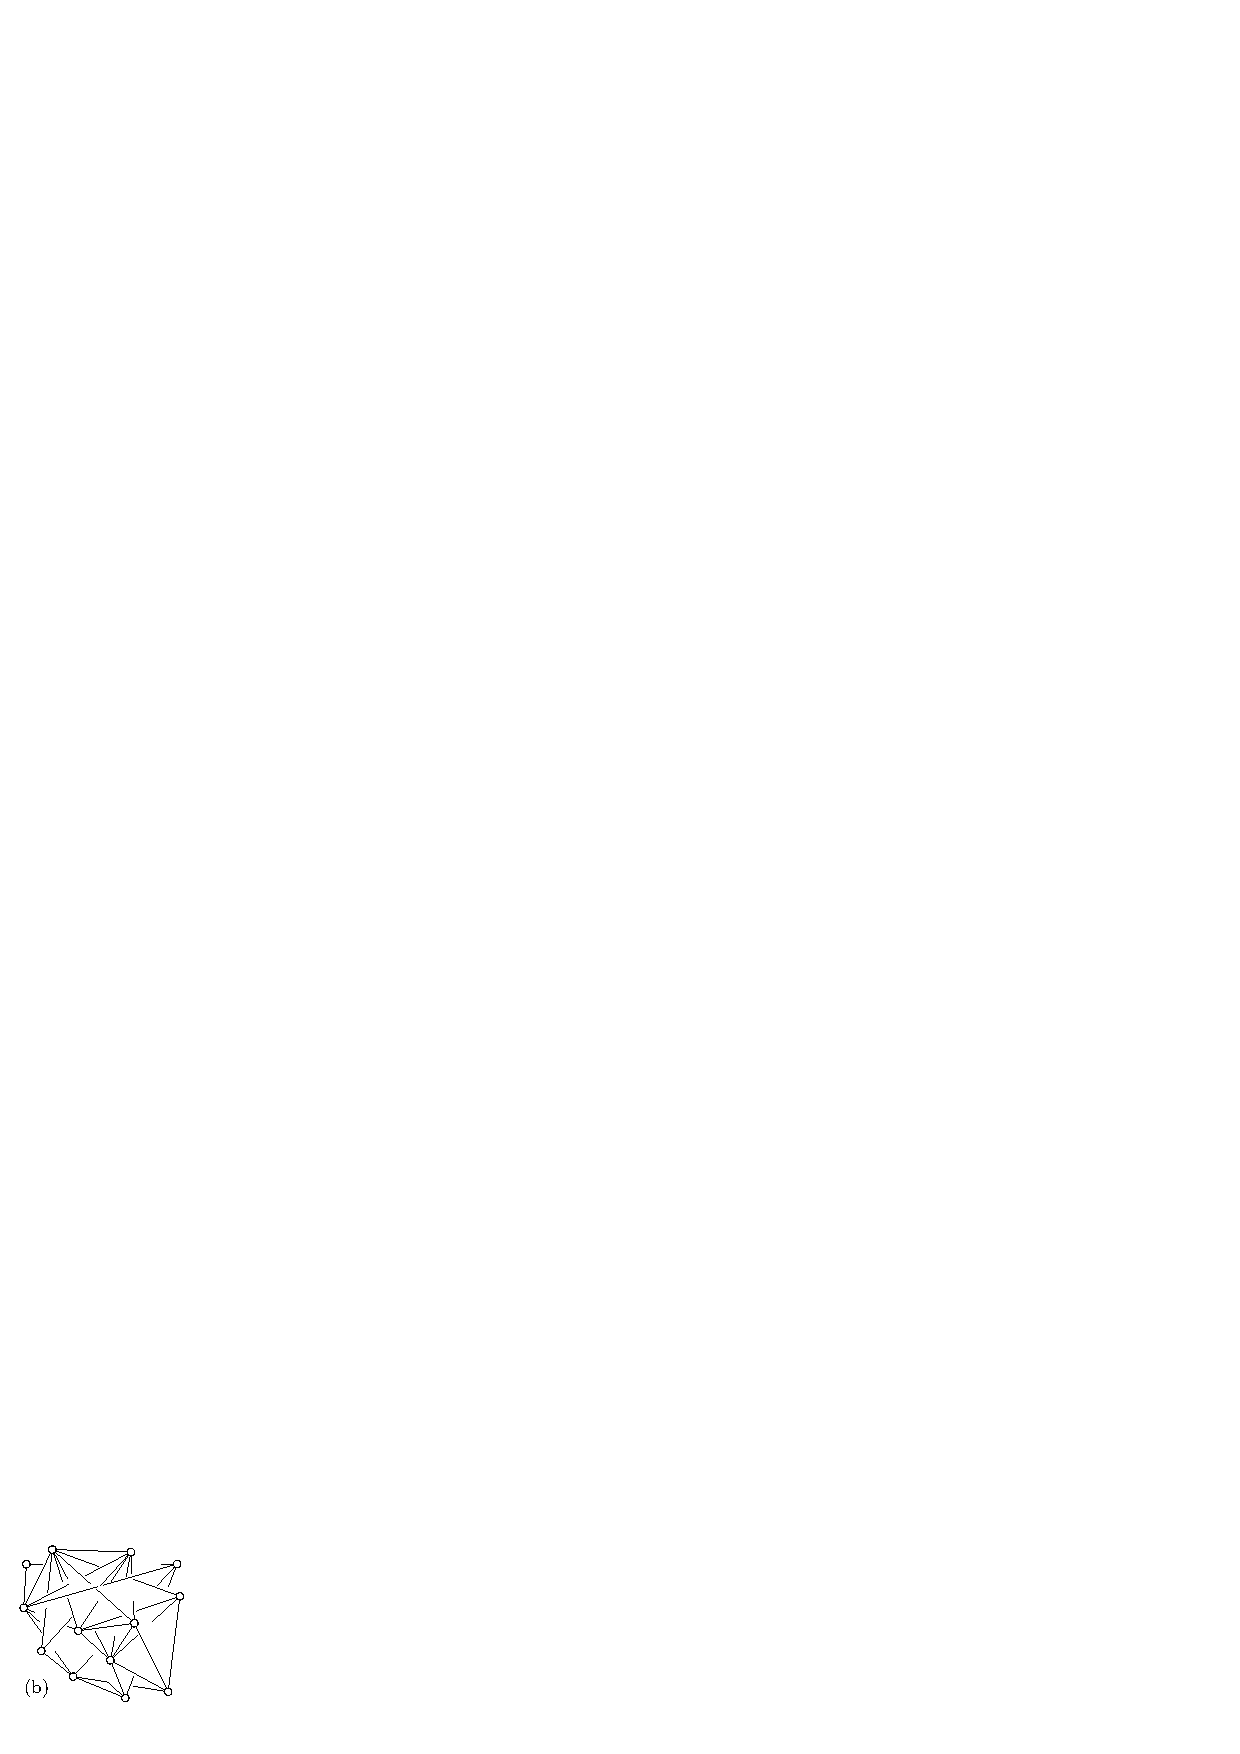
\includegraphics{export_alpha_nontouching}
	\caption{A straight-line graph drawing (a) and a maximum-ink symmetric partial edge drawing (b) of the same graph.}
	\label{fig:examples}
\end{wrapfigure}


The idea of drawing edges only partially has been formalized in graph drawing as follows~\cite{bk-ecbe-12}. 
A \emph{partial edge drawing (PED)} is a graph drawing that maps vertices to points and edges to pairs of crossing-free edge stubs of positive length pointing towards each other.
These edge stubs are obtained by erasing one contiguous central piece of the straight-line segment connecting the two endpoints of each edge.
In other words each straight-line edge is divided into three parts, of which only the two outer ones are drawn, see Fig.~\ref{fig:examples}.
More restricted and better readable~\cite{blmt-pedhmitc-16} variations of PEDs are \emph{symmetric} PEDs, in which both stubs of an edge must have the same length (see Fig.~\ref{fig:examples}(b)), and \emph{homogeneous} PEDs, in which the ratio of the stub length to the total edge length is the same for all edges.
The natural optimization problem in this formal setting is \emph{ink maximization}, i.e., maximizing the total stub length, so that as much information as possible is given in the drawing while all crossings disappear in the negative background space. 


We study the ink maximization problem for symmetric partial edge drawings (SPEDs) with a given geometric input drawing.
This problem is known as \maxsped. 
Bruckdorfer and Kaufmann~\cite{bk-ecbe-12} presented an integer linear program for solving \maxsped. 
Later, Bruckdorfer et al.~\cite{bcgkmn-pped-17} gave an $O(n \log n)$-time algorithm for \maxsped on the class of 2-plane input drawings (no edge has more than two crossings), where $n$ is the number of vertices, and an efficient 2-approximation algorithm for the dual problem of minimizing the amount of erased ink for arbitrary input drawings.
Bruckdorfer~\cite{b-sgh-15} further gives an \NP-hardness proof for \maxsped.

\medskip

\noindent\textbf{Contribution.} We extend the results of Bruckdorfer et al.~\cite{bcgkmn-pped-17} on 2-plane geometric graph drawings to $k$-plane graph drawings for $k > 2$. 
In particular, we show that \maxsped is \NP-hard even for 3-plane input drawings. 
However, for graph drawings whose edge intersection graphs are trees or cacti of maximum degree $k$, we give polynomial-time algorithms for solving \maxsped.





\section{Preliminaries}
%\begin{itemize}
%	\item basic definitions and notation
%	\item segment intersection graph
%	\item alle planaren Graphen können auftreten (insbes. Bäume und Kakteen)
%\end{itemize}
%Input: $k$-plane graph drawing $\Gamma$ of a graph $G$ with edge set $S={s_1, \dots, s_m}$ (set of segments)
%Intersection graph $C=(V,E)$ with $V=S$ and edges if two segments intersect 
%Consider maximum degree of $C$ -- here mostly 3.

Let $ G $ be a \emph{simple graph} with edge set $ S = \{s_1,\dots,s_m\}$ and $ \Gamma $ a straight line drawing of $ G $ in the plane. We call $ \Gamma $ \emph{$ k $-plane} if every edge $ s_i \in S $ is crossed by at most $ k $ other edges from $ S $ in $ \Gamma $. The \emph{intersection graph} $ C = (V,E) $ of $ \Gamma $ is the graph containing a vertex $v_i$ in $ V $ for every $ s_i \in S $ and an edge $ v_i v_j \in E $ between vertices $ v_i, v_j \in V $ if the corresponding edges $ s_i, s_j \in S $ intersect in $ \Gamma $. Observe that the intersection graph $ C $ of a $ k $-plane drawing $ \Gamma $ has maximum degree $ k $. It is known that every planar graph is representable as the intersection graph of line segments~\cite{chalopin2009every}.

\fabian{This part has to be adapted once the intro is fixed}

We define a \emph{partial edge drawing} (\ped) $ \Gamma' $ of $ G $ as a drawing using the same embedding as $ \Gamma $, but edges are drawn as \emph{stubs}, i.e., we do not depict an edge $ s_i \in S $ by a line segment connecting the two vertices, but remove the middle part of the edges such that no two stubs intersect in $ \Gamma' $. We call a \ped $ \Gamma' $ \emph{symmetric} if for every edge $ s_i s_j \in S $ its two stubs have equal lengths in $ \Gamma' $. Finally we define the problem \maxsped as finding a symmetric \ped $ \Gamma' $ of $ G $ where the sum of the lengths of the stubs is maximized. This is also known as ink maximization~\cite{bcgkmn-pped-17}.

\martin{Maybe we don't need the above paragraph as PED, SPED, maxSPED are all somewhat defined in the introduction}

\section{Hardness}
\fabian{Use the reduction from Till Bruckdorfers Dissertation \cite{b-sgh-15}. The Clauses can be modelled as triangles, the Variables as Circles with every second segment connected to a path. Path should have even length, segments are of length four.}

Soeren?


\section{Two Polynomial Cases}

\begin{itemize}
	\item dynamic programming
	\item table entries $T_i(s)$ for $i = 1, \dots, \deg(s)$
	\item $i$ corresponds to increasing stub lengths
	\item stub lengths $l_i(s)$ for $i = 1, \dots, \deg(s)$ (not the pair of stubs)
\end{itemize}

\subsection{Trees}
\fabian{Algorithm running in $O(kn)$ where $ k $ is the max degree of the tree + intersection graph bauen.}

Birgit

\begin{itemize}
	\item segment $s$ with $d$ children $u_1, \dots, u_{d}$ and parent $p(s) = p$.
	\item Assume children are sorted by their intersection points on $s$, i.e., $u_1$ produces stub length $l_1$ etc.
	\item for stub length relating to parent use offset from next longer stub length
\end{itemize}

\subsection{Cacti (of Degree Three)}
\fabian{Algorithm running in $ O(kn) $ + intersection graph bauen.}

\begin{itemize}
	\item seems to work for all cactus graphs
\end{itemize}

\section{Conclusion}


\bibliography{paper}

\end{document}
